\documentclass[aps,pra,twocolumn,superscriptaddress,nofootinbib]{revtex4-2}
\usepackage{amsmath,amssymb}
\usepackage{graphicx}
\usepackage{xcolor}

% AUTO-GENERATED by src/make_numbers.py - do not edit
\newcommand{\rmseLmFiveK}{743}
\newcommand{\biasLmFiveK}{-64}
\newcommand{\rmseLmTenK}{629}
\newcommand{\biasLmTenK}{+39}
\newcommand{\rmseLmTwentyK}{383}
\newcommand{\biasLmTwentyK}{-77}
\newcommand{\rmseLmFortyK}{262}
\newcommand{\biasLmFortyK}{-33}
\newcommand{\rmseLmEightyK}{195}
\newcommand{\biasLmEightyK}{+45}
\newcommand{\rmseLmOneSixtyK}{165}
\newcommand{\biasLmOneSixtyK}{-0}
\newcommand{\rmseLmThreeTwentyK}{109}
\newcommand{\biasLmThreeTwentyK}{+5}
\newcommand{\rmseLmSixFortyK}{59}
\newcommand{\biasLmSixFortyK}{-15}
\newcommand{\rmsePoolFiveK}{439}
\newcommand{\biasPoolFiveK}{+8}
\newcommand{\rmsePoolTenK}{344}
\newcommand{\biasPoolTenK}{+146}
\newcommand{\rmsePoolTwentyK}{272}
\newcommand{\biasPoolTwentyK}{+83}
\newcommand{\rmsePoolFortyK}{176}
\newcommand{\biasPoolFortyK}{+98}
\newcommand{\rmsePoolEightyK}{215}
\newcommand{\biasPoolEightyK}{+185}
\newcommand{\rmsePoolOneSixtyK}{175}
\newcommand{\biasPoolOneSixtyK}{+144}
\newcommand{\rmsePoolThreeTwentyK}{174}
\newcommand{\biasPoolThreeTwentyK}{+151}
\newcommand{\rmsePoolSixFortyK}{146}
\newcommand{\biasPoolSixFortyK}{+125}
\newcommand{\rmsePartFiveK}{465}
\newcommand{\biasPartFiveK}{-11}
\newcommand{\rmsePartTenK}{343}
\newcommand{\biasPartTenK}{+139}
\newcommand{\rmsePartTwentyK}{261}
\newcommand{\biasPartTwentyK}{+16}
\newcommand{\rmsePartFortyK}{146}
\newcommand{\biasPartFortyK}{+16}
\newcommand{\rmsePartEightyK}{151}
\newcommand{\biasPartEightyK}{+105}
\newcommand{\rmsePartOneSixtyK}{123}
\newcommand{\biasPartOneSixtyK}{+73}
\newcommand{\rmsePartThreeTwentyK}{123}
\newcommand{\biasPartThreeTwentyK}{+89}
\newcommand{\rmsePartSixFortyK}{95}
\newcommand{\biasPartSixFortyK}{+61}
\newcommand{\rmseNetFiveK}{455}
\newcommand{\biasNetFiveK}{-88}
\newcommand{\rmseNetTenK}{427}
\newcommand{\biasNetTenK}{-63}
\newcommand{\rmseNetTwentyK}{309}
\newcommand{\biasNetTwentyK}{-63}
\newcommand{\rmseNetFortyK}{222}
\newcommand{\biasNetFortyK}{-104}
\newcommand{\rmseNetEightyK}{240}
\newcommand{\biasNetEightyK}{-96}
\newcommand{\rmseNetOneSixtyK}{219}
\newcommand{\biasNetOneSixtyK}{-94}
\newcommand{\rmseNetThreeTwentyK}{188}
\newcommand{\biasNetThreeTwentyK}{-78}
\newcommand{\rmseNetSixFortyK}{198}
\newcommand{\biasNetSixFortyK}{-101}
\newcommand{\ratioLmPoolFiveK}{1.69}
\newcommand{\ratioLmPoolTenK}{1.83}
\newcommand{\ratioLmPoolTwentyK}{1.41}
\newcommand{\ratioLmPoolFortyK}{1.49}
\newcommand{\ratioLmPoolEightyK}{0.91}
\newcommand{\ratioLmPoolOneSixtyK}{0.94}
\newcommand{\ratioLmPoolThreeTwentyK}{0.63}
\newcommand{\ratioLmPoolSixFortyK}{0.41}
\newcommand{\crlbFreeFiveK}{744}
\newcommand{\crlbJointFiveK}{419}
\newcommand{\crlbFreeTenK}{526}
\newcommand{\crlbJointTenK}{297}
\newcommand{\crlbFreeTwentyK}{372}
\newcommand{\crlbJointTwentyK}{210}
\newcommand{\crlbFreeFortyK}{263}
\newcommand{\crlbJointFortyK}{148}
\newcommand{\crlbFreeEightyK}{186}
\newcommand{\crlbJointEightyK}{105}
\newcommand{\crlbFreeOneSixtyK}{131}
\newcommand{\crlbJointOneSixtyK}{74}
\newcommand{\crlbFreeThreeTwentyK}{93}
\newcommand{\crlbJointThreeTwentyK}{52}
\newcommand{\crlbFreeSixFortyK}{66}
\newcommand{\crlbJointSixFortyK}{37}
\newcommand{\lawALm}{785.3}
\newcommand{\lawBLm}{27.8}
\newcommand{\lawFitLm}{32.6}
\newcommand{\lawAPool}{416.8}
\newcommand{\lawBPool}{156.2}
\newcommand{\lawFitPool}{18.9}
\newcommand{\crossoverReps}{9.1e+04}
\newcommand{\crossoverRepsRounded}{9}
\newcommand{\photonGainFactor}{3.55}
\newcommand{\envAMean}{0.127}
\newcommand{\envAStd}{0.005}
\newcommand{\envCMean}{0.889}
\newcommand{\envCStd}{0.006}
\newcommand{\envTstarMean}{5.404}
\newcommand{\envTstarStd}{0.294}
\newcommand{\envpMean}{2.014}
\newcommand{\envpStd}{0.423}
\newcommand{\envphiMean}{-0.044}
\newcommand{\envphiStd}{0.123}
\newcommand{\sysMedianAbs}{44}
\newcommand{\sysMin}{-107}
\newcommand{\sysMax}{+139}
\newcommand{\ctrlLmFiveK}{520.7}
\newcommand{\ctrlPoolFiveK}{374.5}
\newcommand{\ctrlPartFiveK}{414.4}
\newcommand{\ctrlLmTenK}{415.8}
\newcommand{\ctrlPoolTenK}{270.0}
\newcommand{\ctrlPartTenK}{280.8}
\newcommand{\ctrlLmFortyK}{248.8}
\newcommand{\ctrlPoolFortyK}{257.7}
\newcommand{\ctrlPartFortyK}{271.2}
\newcommand{\ctrlLmOneSixtyK}{91.3}
\newcommand{\ctrlPoolOneSixtyK}{235.9}
\newcommand{\ctrlPartOneSixtyK}{235.2}
\newcommand{\ctrlLmSixFortyK}{51.7}
\newcommand{\ctrlPoolSixFortyK}{217.8}
\newcommand{\ctrlPartSixFortyK}{235.3}
\newcommand{\etaLmFiveK}{1.82}
\newcommand{\etaPoolFiveK}{1.08}
\newcommand{\etaLmTenK}{2.18}
\newcommand{\etaPoolTenK}{1.19}
\newcommand{\etaLmTwentyK}{1.88}
\newcommand{\etaPoolTwentyK}{1.33}
\newcommand{\etaLmFortyK}{1.81}
\newcommand{\etaPoolFortyK}{1.22}
\newcommand{\etaLmEightyK}{1.91}
\newcommand{\etaPoolEightyK}{2.11}
\newcommand{\etaLmOneSixtyK}{2.29}
\newcommand{\etaPoolOneSixtyK}{2.43}
\newcommand{\etaLmThreeTwentyK}{2.15}
\newcommand{\etaPoolThreeTwentyK}{3.41}
\newcommand{\etaLmSixFortyK}{1.65}
\newcommand{\etaPoolSixFortyK}{4.04}
\newcommand{\nTau}{300}
\newcommand{\nCols}{40}
\newcommand{\nSheets}{8}
\newcommand{\tauMax}{6.0}
\newcommand{\bMax}{42.9}
\newcommand{\rMinK}{5}
\newcommand{\rMaxK}{640}
\newcommand{\tauOffNs}{18.6}
\newcommand{\tauStep}{20}
\newcommand{\bStep}{1071.4}
\newcommand{\nBins}{512}
\newcommand{\WResid}{8}
\newcommand{\tauOffSigmaNs}{2.6}
\newcommand{\nSeedsNetSet}{5}
\newcommand{\netSteps}{30000}
\newcommand{\rmseNetSetFiveK}{504}
\newcommand{\medNetSetFiveK}{381}
\newcommand{\rmseNetSetTenK}{387}
\newcommand{\medNetSetTenK}{253}
\newcommand{\rmseNetSetTwentyK}{289}
\newcommand{\medNetSetTwentyK}{149}
\newcommand{\rmseNetSetFortyK}{172}
\newcommand{\medNetSetFortyK}{100}
\newcommand{\rmseNetSetEightyK}{139}
\newcommand{\medNetSetEightyK}{86}
\newcommand{\rmseNetSetOneSixtyK}{113}
\newcommand{\medNetSetOneSixtyK}{74}
\newcommand{\rmseNetSetThreeTwentyK}{88}
\newcommand{\medNetSetThreeTwentyK}{48}
\newcommand{\rmseNetSetSixFortyK}{66}
\newcommand{\medNetSetSixFortyK}{37}
\newcommand{\phaseConcFiveK}{0.955}
\newcommand{\phaseConcTenK}{0.971}
\newcommand{\phaseConcTwentyK}{0.989}
\newcommand{\phaseConcFortyK}{0.985}
\newcommand{\phaseConcEightyK}{0.989}
\newcommand{\phaseConcOneSixtyK}{0.991}
\newcommand{\phaseConcThreeTwentyK}{0.993}
\newcommand{\phaseConcSixFortyK}{0.992}
\newcommand{\pJointVsLmFiveK}{5.9\times10^{-2}}
\newcommand{\pPartVsLmFiveK}{9.2\times10^{-2}}
\newcommand{\pNetVsLmFiveK}{9.8\times10^{-2}}
\newcommand{\pJointVsLmTenK}{1.7\times10^{-3}}
\newcommand{\pPartVsLmTenK}{1.6\times10^{-3}}
\newcommand{\pNetVsLmTenK}{7.2\times10^{-2}}
\newcommand{\pJointVsLmTwentyK}{3.3\times10^{-2}}
\newcommand{\pPartVsLmTwentyK}{9.6\times10^{-3}}
\newcommand{\pNetVsLmTwentyK}{3.3\times10^{-1}}
\newcommand{\pJointVsLmFortyK}{4.1\times10^{-3}}
\newcommand{\pPartVsLmFortyK}{1.9\times10^{-5}}
\newcommand{\pNetVsLmFortyK}{9.1\times10^{-2}}
\newcommand{\pJointVsLmEightyK}{2.4\times10^{-1}}
\newcommand{\pPartVsLmEightyK}{1.4\times10^{-1}}
\newcommand{\pNetVsLmEightyK}{7.0\times10^{-2}}
\newcommand{\pJointVsLmOneSixtyK}{2.9\times10^{-1}}
\newcommand{\pPartVsLmOneSixtyK}{1.8\times10^{-1}}
\newcommand{\pNetVsLmOneSixtyK}{3.3\times10^{-1}}
\newcommand{\pJointVsLmThreeTwentyK}{5.0\times10^{-4}}
\newcommand{\pPartVsLmThreeTwentyK}{2.8\times10^{-1}}
\newcommand{\pNetVsLmThreeTwentyK}{8.1\times10^{-4}}
\newcommand{\pJointVsLmSixFortyK}{2.0\times10^{-5}}
\newcommand{\pPartVsLmSixFortyK}{4.9\times10^{-3}}
\newcommand{\pNetVsLmSixFortyK}{4.1\times10^{-6}}
\newcommand{\acfLagOneFiveK}{-0.010}
\newcommand{\acfLagOneFortyK}{-0.010}
\newcommand{\acfLagOneSixFortyK}{+0.004}
\newcommand{\crossoverCIlow}{4.9}
\newcommand{\crossoverCIhigh}{12.9}
\newcommand{\crossoverMedianK}{89}
\newcommand{\attribAllSharedRmse}{371}
\newcommand{\attribAllSharedBias}{-85}
\newcommand{\attribTFreeRmse}{73}
\newcommand{\attribTFreeBias}{-10}
\newcommand{\attribPFreeRmse}{371}
\newcommand{\attribPFreeBias}{-85}
\newcommand{\attribAFreeRmse}{371}
\newcommand{\attribAFreeBias}{-85}
\newcommand{\nSeedsAblation}{5}
\newcommand{\rmseAblFiveK}{559}
\newcommand{\rmseAblTenK}{402}
\newcommand{\rmseAblTwentyK}{285}
\newcommand{\rmseAblFortyK}{189}
\newcommand{\rmseAblEightyK}{145}
\newcommand{\rmseAblOneSixtyK}{130}
\newcommand{\rmseAblThreeTwentyK}{96}
\newcommand{\rmseAblSixFortyK}{83}


\newcommand{\dB}{\delta B}
\newcommand{\etaS}{\eta}
\newcommand{\mus}{\,\mu\mathrm{s}}
\newcommand{\muT}{\,\mu\mathrm{T}}

\begin{document}

\title{Photon-budget-dependent estimation strategy for\\
nitrogen-vacancy Ramsey magnetometry}

\author{Author list to be finalized}
\affiliation{}

\date{\today}

\begin{abstract}
Estimating a static magnetic field from a Ramsey fringe is usually discussed as a problem
of photon shot noise, as if the inference itself were free. Working with a real
nitrogen-vacancy (NV) diamond data set that spans a $128\times$ range of photon budget
($\rMinK\times10^{3}$ to $\rMaxK\times10^{3}$ repetitions per delay point, $\nTau$-point
sweep, $\nCols$ field settings), we show that the sensitivity-optimal \emph{inference
strategy} changes with the budget. Per-trace maximum-likelihood fitting is essentially
efficient against its own Cram\'er--Rao bound at every budget ($\rmseLmFiveK$~nT at
$\rMinK$k repetitions against a free-envelope bound of $\crlbFreeFiveK$~nT), yet sits a
factor $\ratioLmPoolFiveK$ above the bound that becomes available when the instrument's
shared nuisance structure, one relaxation envelope and one phase frame for a whole field
sweep, is pooled across the sweep's field settings. Pooling is not free: it carries a
\emph{bias floor} set by the measured inhomogeneity of the relaxation envelope
($T_2^{*}=\envTstarMean\pm\envTstarStd\mus$ across the $\nCols$ columns), which is invisible
while photons are scarce and dominant once they are not. Both estimators obey a two-term
law $\dB(r)=\sqrt{A^{2}(5000/r)+b^{2}}$ with $A=\lawALm$~nT, $b=\lawBLm$~nT for per-trace
fitting and $A=\lawAPool$~nT, $b=\lawBPool$~nT for pooled fitting, crossing at
$r^{*}\approx\crossoverRepsRounded\times10^{4}$ repetitions. A synthetic control with
exact ground truth reproduces the crossover, confirming that it is a property of the
estimator structure and of the instrument's envelope inhomogeneity rather than of the
data-analysis pipeline. An amortized neural estimator trained across the whole budget
range selects its own degree of pooling: it attains the best measured precision of any
estimator at and above $80$k repetitions and stays within $\sim\!25\%$ of the pooled bound
at the lowest budget, without being told which parameters are shared. The crossover sets
an operationally useful rule: spend photons until the pooled estimator's bias floor is
reached, then stop sharing.
\end{abstract}

\maketitle

\section{Introduction}

Magnetometry with nitrogen-vacancy (NV) centres in diamond has become a workhorse of
quantum sensing~\cite{Taylor2008,Maze2008,Balasubramanian2008,Degen2017,Barry2020}. In the
Ramsey protocol, a superposition of the NV spin states accumulates a field-dependent phase
$\phi=\gamma B\tau$ over a free precession time $\tau$, and the resulting population
oscillation is read out optically. Repeating over a grid of delays yields a damped fringe
whose oscillation frequency fixes $B$. The sensitivity of such a measurement is
conventionally written $\etaS=\dB\sqrt{t_{\rm total}}$, where $\dB$ is the field
uncertainty and $t_{\rm total}$ the accumulation time of the data used~\cite{Barry2020}.

Almost all of the sensitivity discussion in the literature concerns the \emph{hardware and
protocol} side of that expression: contrast, collection efficiency, coherence
time~\cite{Barry2020,Rondin2014}, or the choice of which delay times to
measure~\cite{Santagati2019}. The inference side, namely how close a practical estimator
actually comes to the information-theoretic bound for a given finite data set, is rarely
the headline, even though it sets the achievable sensitivity whenever photons are scarce.
Learned estimators for NV data have appeared
recently~\cite{Guo2025,NVRNet2026,Haim2025,Daniel2026,Youssry2026}, but they are usually
benchmarked on simulations or against weakly tuned classical baselines, and the
simulation-to-reality gap is repeatedly identified as the central
difficulty~\cite{NVRNet2026,Daniel2026}.

In this work we ask the estimator-side question directly, on real data, with a fixed
measurement protocol. We use a DC Ramsey data set in which the same $\nCols$ field
settings are measured on $\nSheets$ sheets that differ only in the number of repetitions
per delay point ($\rMinK\times10^{3}$ to $\rMaxK\times10^{3}$, thus a $128\times$ photon
range), always with the full $\nTau$-point delay sweep. This lets us compare estimators at
\emph{matched photon budget}. We deliberately do not study sparse or adaptive delay
sampling: the sweep is fixed and only the photon budget varies.

Our main finding is that the optimal estimator is not the same at all budgets. A per-trace
fit, with six free parameters per fringe, is efficient against its own Cram\'er--Rao bound,
but that bound is inflated by the need to determine the fringe's nuisance parameters from a
single trace. Pooling the nuisance parameters across the $\nCols$ field settings of a sweep
moves the bound down by a factor close to two. However, the pooling assumption is
imperfect: the relaxation envelope genuinely varies across the field range, and the
resulting model error acts as a bias floor that dominates the photon-limited term above
$r^{*}\approx\crossoverRepsRounded\times10^{4}$ repetitions. The sensitivity-optimal
strategy is therefore budget-dependent, and we quantify its crossover.

\section{Experiment and data}

The data set consists of DC Ramsey measurements on an NV ensemble, provided as $\nSheets$
sheets of a $\nTau\times\nCols$ array. Rows are delay times $\tau_i = \tauStep\,i$ with
$i=1,\dots,\nTau$ and a step of $20$~ns, i.e.\ $0.02$ to $\tauMax\mus$. Columns are applied
fields $B_n = \bStep\,n$ with $n=1,\dots,\nCols$, i.e.\ $1071.4$~nT steps covering $1.07$ to
$\bMax\muT$. Each sheet corresponds to a different number of laser--microwave repetitions
per delay point, $r\in\{5,10,20,40,80,160,320,640\}\times10^{3}$; the signal-to-noise ratio
scales with $r$ as expected for shot noise. All evaluations in this paper use the real
traces; no synthetic data appears in any reported performance number. Synthetic traces are
used only to train the neural estimator described in Sec.~\ref{sec:net} and, with
\emph{exact} ground truth, in the control experiment of Sec.~\ref{sec:control}.

We use the standard model for a Ramsey fringe with a stretched-exponential envelope,
\begin{equation}
s(\tau)=C+A\,e^{-(\tau/T_2^{*})^{p}}\cos\!\big[\gamma B(\tau+\tau_{\rm off})+\phi_0\big],
\label{eq:model}
\end{equation}
with $\gamma=2\pi\times28\times10^{-6}$~rad$/(\mu{\rm s}\,{\rm nT})$. Two instrument
conventions are adopted from prior work on the same apparatus and are treated as known
throughout: a timing offset $\tau_{\rm off}=\tauOffNs\pm\tauOffSigmaNs$~ns
\cite{L1companion}, and the global phase frame of a session, i.e.\ the instrument phase
$\phi_0$ is common to all field settings of one sweep, as we verify below.

\emph{Noise.} A robust per-point noise estimate (standard deviation of the three-point
second difference, divided by $\sqrt 6$) gives $0.2079,0.1500,0.1072,0.0745,0.0533,0.0370,
0.0263,0.0183$ for the eight sheets, matching the shot-noise law
$\sigma(r)=0.207\sqrt{5000/r}$ to within $1$--$3.5\%$. We use that law wherever a noise
level is needed.

\emph{Envelope population.} Fitting Eq.~\eqref{eq:model} to the $\nCols$ columns of the
highest-budget sheet gives $A=\envAMean\pm\envAStd$, $C=\envCMean\pm\envCStd$,
$T_2^{*}=\envTstarMean\pm\envTstarStd\mus$, $p=\envpMean\pm\envpStd$ and
$\phi_0=\envphiMean\pm\envphiStd$~rad (Fig.~\ref{fig:env}). The phase scatter is consistent
with a common instrument phase: the circular concentration of $\phi_0$ across columns is
$\phaseConcFiveK$ at $\rMinK$k, $\phaseConcTenK$ at $10$k and $\phaseConcThreeTwentyK$--$\phaseConcSixFortyK$ at $320$k and $\rMaxK$k
repetitions. The relaxation time, by contrast, genuinely varies by $\pm5\%$ across the
field range, a fact that will matter in Sec.~\ref{sec:control}.

\emph{Ground truth and its systematic.} The applied field is the nominal value $B_n$.
Fitting the highest-budget sheet column by column, the fitted fields deviate from the
nominal values by $\sysMedianAbs$~nT (median absolute deviation, columns 7--40; range
$\sysMin$ to $\sysMax$~nT). This is a property of the magnet and its calibration rather
than of any estimator, and it is why all comparisons below are made against $B_n$ while its
$\sim\!50$~nT scale is stated explicitly: at the two highest budgets the per-trace
statistical error approaches this scale, and we mark that boundary in the figures.

\section{Models, bounds and estimators}

\subsection{Estimation task}

We estimate an unknown field from one full $\nTau$-point trace. To exclude any possibility
of scoring an estimator by information contained in the experimental set point, the task is
\emph{blind}: the estimator is given $B\in[0.5,45]\muT$ and nothing else about the field.
All classical estimators are initialised identically from a blind FFT$+$Rife~\cite{Rife1970}
estimate of the same trace, which is standard practice for fringe fitting, so that
differences between estimators reflect the refinement step alone. We report results for
columns $7$--$40$ ($B\ge7.5\muT$, at least $\sim\!1.3$ oscillations within the sweep) as
the primary region. Columns $1$--$6$ are treated separately: those sub-cycle records are
not identifiable per trace at low budget by any method we tried, and their calibrated
treatment belongs to companion work~\cite{L1companion}.

\subsection{Cram\'er--Rao bounds and why pooling moves them}

For a fixed sweep, three bounds are relevant. If the envelope $(A,C,T_2^{*},p,\phi_0)$ is
known, the field bound $\sigma_B^{\rm known}$ follows from the Fisher information
$\mathcal{I}_B=\sum_i(\partial s_i/\partial B)^2/\sigma^2$. If the envelope is free, the
bound inflates to $\sigma_B^{\rm free}$, because six parameters must be determined from the
same trace. If instead the envelope is \emph{shared} across the $\nCols$ field settings of
a sweep while each column keeps its own field, the relevant bound
$\sigma_B^{\rm joint}$ follows from the joint Fisher matrix: the nuisance cost is paid once
for the whole session rather than once per trace. For the measured trace geometry at
$\rMinK$k repetitions these are $\crlbFreeFiveK$~nT (free, per trace) and
$\crlbJointFiveK$~nT (joint, $\nCols$ columns). The ratio
$\sigma_B^{\rm free}/\sigma_B^{\rm joint}\approx1.8$ is set by the fringe geometry, namely
the number of oscillations, the decay and the sampling, and is essentially independent of
the photon budget.

The scientific content of this paper is what happens when these bounds are confronted with
real estimators on real data, including the fact that the shared-envelope model is not
exactly true for a real instrument.

\subsection{Estimators}

\emph{Per-trace fitting} (\texttt{lm}). Levenberg--Marquardt least squares with
multi-start over the initial phase, fitting all six parameters of Eq.~\eqref{eq:model} from
the FFT estimate, with $25$ starts inside the blind window. Doubling the number of starts
changes the result by less than $0.1$~nT.

\emph{Session-pooled fitting} (\texttt{pool}). A single least-squares problem over all
$\nCols$ columns of a sweep: one $(A,C,T_2^{*},p,\phi_0)$ shared by every column and one
field per column. This is the classical estimator that exploits the shared instrument
structure, and its bound is $\sigma_B^{\rm joint}$.

\emph{Partial pooling} (\texttt{part}). As above, but each column keeps its own $T_2^{*}$
while $A$, $C$, $p$ and $\phi_0$ remain shared. This structure follows the measured
instrument: the phase frame is genuinely common, the relaxation time is not.

\emph{Amortized network.} See Sec.~\ref{sec:net}.

\subsection{Metrics}

We report the root-mean-square error over the $\nCols$ real traces of a sheet, which is a
$\sigma$-equivalent statistic, together with the signed bias and a percentile bootstrap
confidence interval over columns. A quoted median is related to the Gaussian-equivalent
$\sigma$ by the usual factor $0.674$. Each estimator is compared with its \emph{own} bound:
the free-envelope bound for per-trace fitting and the joint bound for the pooled
estimators. The sensitivity uses a declared per-point overhead,
$t_{\rm total}(r)=r\sum_i(\tau_i+t_{\rm ovh})$, for $t_{\rm ovh}\in\{0.5,1,2\}$~$\mu$s.
All reported fractions and rankings are overhead-independent, because every estimator is
charged the same session time.

\section{Results}

\subsection{Both estimators are efficient, but against different bounds}

Figure~\ref{fig:ladder} and Table~\ref{tab:ladder} give the central measurement. In the
primary region, per-trace fitting attains $\rmseLmFiveK$~nT at $\rMinK$k repetitions against
its own free-envelope bound of $\crlbFreeFiveK$~nT, an efficiency of $1.0$--$1.3$ across the
whole budget ladder: the classical fitter is essentially not improvable by a better
optimiser. Session pooling attains $\rmsePoolFiveK$~nT against a joint bound of
$\crlbJointFiveK$~nT, also efficient. The pooled estimator is better by a factor
$\ratioLmPoolFiveK$ at $\rMinK$k repetitions ($\ratioLmPoolTenK$ at $10$k), and that factor is
the same one by which pooling lowers the bound. Pooling therefore does not recover lost
efficiency; it changes the bound. This is the first result: at low photon budget the
achievable precision is limited by the identifiability of the field jointly with the
instrument's nuisance parameters, not by the optimiser.

\begin{table}[t]
\caption{Field RMSE (nT) over the real columns 7--40 as a function of repetitions per delay
point: per-trace LM, session pooling (shared envelope), partial pooling (per-column
$T_2^{*}$) and the amortized session-conditioned network. Values are generated from
\texttt{results/analysis\_v2.json} by \texttt{src/make\_numbers.py}.}
\label{tab:ladder}
\begin{ruledtabular}
\begin{tabular}{r c c c c}
$r$ & \texttt{lm} & \texttt{pool} & \texttt{part} & network \\
\hline
$\rMinK$k & \rmseLmFiveK & \rmsePoolFiveK & \rmsePartFiveK & \rmseNetSetFiveK \\
$10$k & \rmseLmTenK & \rmsePoolTenK & \rmsePartTenK & \rmseNetSetTenK \\
$20$k & \rmseLmTwentyK & \rmsePoolTwentyK & \rmsePartTwentyK & \rmseNetSetTwentyK \\
$40$k & \rmseLmFortyK & \rmsePoolFortyK & \rmsePartFortyK & \rmseNetSetFortyK \\
$80$k & \rmseLmEightyK & \rmsePoolEightyK & \rmsePartEightyK & \rmseNetSetEightyK \\
$160$k & \rmseLmOneSixtyK & \rmsePoolOneSixtyK & \rmsePartOneSixtyK & \rmseNetSetOneSixtyK \\
$320$k & \rmseLmThreeTwentyK & \rmsePoolThreeTwentyK & \rmsePartThreeTwentyK & \rmseNetSetThreeTwentyK \\
$\rMaxK$k & \rmseLmSixFortyK & \rmsePoolSixFortyK & \rmsePartSixFortyK & \rmseNetSetSixFortyK \\
\end{tabular}
\end{ruledtabular}
\end{table}

\begin{figure}[t]
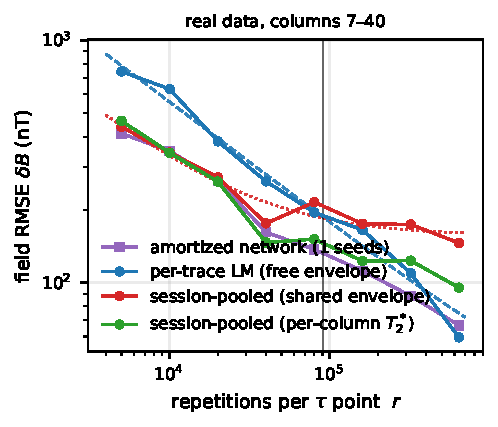
\includegraphics[width=\columnwidth]{figures/fig1_ladder.pdf}
\caption{Field RMSE against repetitions per delay point, real data, columns 7--40.
Markers are the measured estimators; dashed and dotted lines are the two-term law of
Eq.~\eqref{eq:law} fitted to the per-trace and pooled ladders. The vertical line marks the
crossover $r^{*}$.}
\label{fig:ladder}
\end{figure}

\subsection{The crossover law}

Table~\ref{tab:ladder} also shows the reversal: above $\sim\!80$k repetitions the pooled
estimator stops improving and is overtaken by per-trace fitting. The reason is visible in
the estimator bias (Fig.~\ref{fig:bias}). The per-trace bias is consistent with zero at
every budget, whereas the pooled estimator acquires a positive bias that grows with the
budget ($\biasPoolEightyK$~nT at $80$k, $\biasPoolSixFortyK$~nT at $\rMaxK$k): the shared model
becomes progressively more wrong as the statistical error shrinks.

The whole ladder is described by a two-term law,
\begin{equation}
\dB(r)=\sqrt{A^{2}\,(5000/r)+b^{2}},
\label{eq:law}
\end{equation}
in which $A$ is the photon-limited coefficient and $b$ a budget-independent floor. Fitting
the measured ladders gives $A=\lawALm$~nT and $b=\lawBLm$~nT for per-trace fitting (fit rms
$\lawFitLm$~nT) and $A=\lawAPool$~nT and $b=\lawBPool$~nT for pooled fitting (fit rms
$\lawFitPool$~nT). The photon-limited coefficients differ by the bound ratio,
$(A_{\rm lm}/A_{\rm pool})^{2}=\photonGainFactor$: pooling is worth a factor
$\sqrt{\photonGainFactor}$ in precision while photons are scarce, while its floor
$b_{\rm pool}=\lawBPool$~nT eventually costs more than it buys. Equating the two curves
gives the crossover $r^{*}\approx\crossoverReps$ repetitions. Expressed operationally: to
reach the precision that pooled inference achieves at $\rMinK\times10^{3}$ repetitions,
per-trace fitting needs $\photonGainFactor$ times more repetitions; above
$\crossoverRepsRounded\times10^{4}$ repetitions the ordering reverses and per-trace fitting
is the better choice.

\begin{figure}[t]
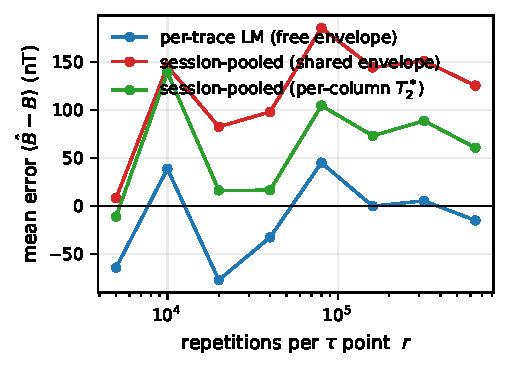
\includegraphics[width=\columnwidth]{figures/fig2_bias.pdf}
\caption{Signed mean error against photon budget for the three classical estimators, real
data, columns 7--40. The pooled estimators acquire a growing bias while per-trace fitting
stays consistent, which is the mechanism behind the crossover of Fig.~\ref{fig:ladder}.}
\label{fig:bias}
\end{figure}

\subsection{Mechanism: a bias floor set by envelope inhomogeneity}
\label{sec:control}

The crossover is a statement about estimators, so it must be reproducible with exact ground
truth. We therefore generated synthetic sessions from Eq.~\eqref{eq:model} with per-column
envelopes drawn from the measured population, exact known fields and the measured shot-noise
levels, and repeated the comparison (Fig.~\ref{fig:control}). The crossover is reproduced:
pooled fitting wins by $1.4\times$ at $\rMinK$k repetitions ($\ctrlPoolFiveK$ versus
$\ctrlLmFiveK$~nT) and loses by $4.2\times$ at $\rMaxK$k ($\ctrlPoolSixFortyK$ versus
$\ctrlLmSixFortyK$~nT), with the pooled error flattening at $\sim\!\lawBPool$~nT, the same floor
as in the fit to the real ladder. Because the synthetic experiment has no measurement
systematics, no calibration error and no data-pipeline artefacts, the floor must come from
the model: it is the envelope inhomogeneity of Fig.~\ref{fig:env} entering through the
shared-envelope assumption. Partial pooling, which lets $T_2^{*}$ vary per column, lowers
the floor ($\ctrlPartSixFortyK$~nT at $\rMaxK$k) and shifts the crossover beyond the measured
range, exactly as expected if the floor is caused by the constraint that is relaxed.

\begin{figure}[t]
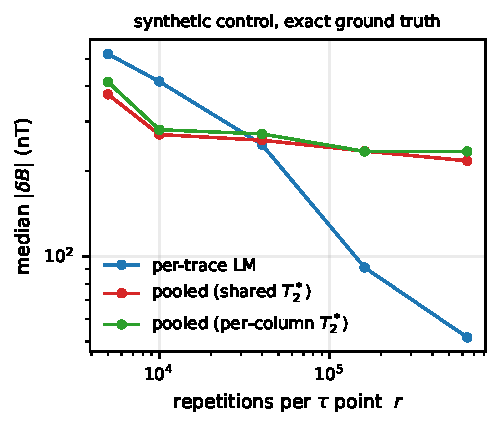
\includegraphics[width=\columnwidth]{figures/fig3_control.pdf}
\caption{Synthetic control with exact ground truth and the measured envelope population.
Median field error against budget for per-trace fitting, full pooling and partial pooling.
Note the reversal between the lowest and the highest budgets.}
\label{fig:control}
\end{figure}

\begin{figure}[t]
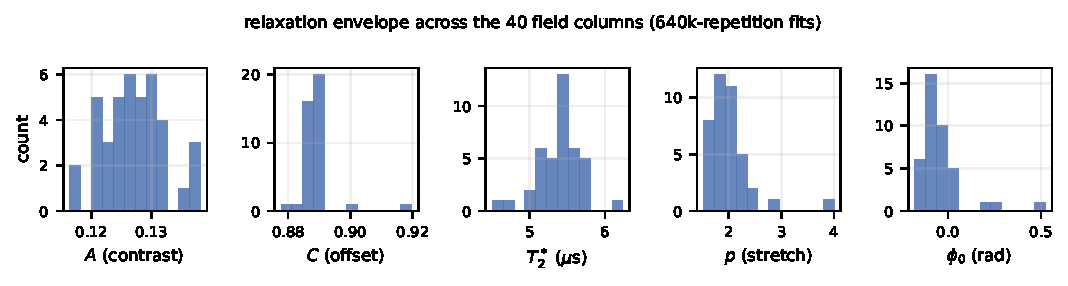
\includegraphics[width=\columnwidth]{figures/fig4_envelope.pdf}
\caption{Relaxation envelope measured across the $\nCols$ field settings from the
highest-budget sheet. The phase $\phi_0$ is essentially common (circular concentration
$\ge0.99$), whereas the relaxation time varies by $\pm5\%$; that inhomogeneity sets the
pooled bias floor.}
\label{fig:env}
\end{figure}

\subsection{Sensitivity}

With the declared accounting $t_{\rm total}(r)=r\sum_i(\tau_i+t_{\rm ovh})$, the sensitivity
$\etaS=\dB\sqrt{t_{\rm total}}$ at $t_{\rm ovh}=1$~$\mu$s reads
$\etaS_{\rm pool}=\etaPoolFiveK\times10^{6}$ and
$\etaS_{\rm lm}=\etaLmFiveK\times10^{6}$~nT$\sqrt{\mu{\rm s}}$ at $\rMinK$k repetitions
(Fig.~\ref{fig:eta}), and $\etaS_{\rm pool}=\etaPoolSixFortyK\times10^{6}$ versus
$\etaS_{\rm lm}=\etaLmSixFortyK\times10^{6}$ at $\rMaxK$k. The ranking inverts at the same
crossover as the field error, and it is unchanged under
$t_{\rm ovh}\in\{0.5,1,2\}$~$\mu$s, because every estimator is charged the same session
time: the overhead rescales $\etaS$ without reordering the estimators. This is the practical
form of our result. For a fixed sweep and a fixed photon budget there is a best inference
strategy, and it changes at $r^{*}$.

\begin{figure}[t]
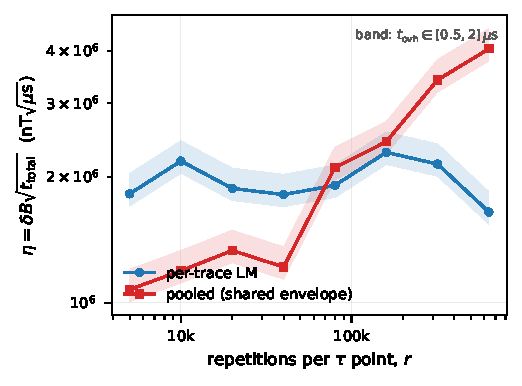
\includegraphics[width=\columnwidth]{figures/fig5_eta.pdf}
\caption{Sensitivity $\etaS=\dB\sqrt{t_{\rm total}}$ against repetitions per delay point for
per-trace and pooled inference, with the per-point overhead $t_{\rm ovh}$ varied over $0.5$,
$1$ and $2$~$\mu$s. The crossover is overhead-independent.}
\label{fig:eta}
\end{figure}

\subsection{An amortized estimator that chooses its own pooling}
\label{sec:net}

The two-term law tells an experimenter \emph{which} strategy to use, but it requires the
instrument's envelope statistics and the photon budget to be known in advance. We therefore
trained a neural estimator that spans the entire budget range with a single set of weights
and asked how close it comes to the best classical strategy at each budget. The network
reads all $\nCols$ traces of a session and, for each column, predicts a posterior over a
correction to the blind FFT$+$Rife estimate of that same trace,
$q(\delta\,|\,\text{trace},\log\sigma)$. The session context enters through a
permutation-invariant attention block, so the network can pool as much or as little as the
data support. Training uses instrument-anchored synthetic sessions (measured envelope
population, measured noise law, blind fields) and evaluation is on the real traces; no real
low-budget trace is used in training. Reported values are the median over
\nSeedsNetSet{} training seeds.

Table~\ref{tab:ladder} and Fig.~\ref{fig:ladder} show the outcome. Without being told which
parameters are shared, the network lands close to pooled inference at the lowest budgets
($\rmseNetSetFiveK$~nT at $\rMinK$k, i.e.\ $27\%$ better than per-trace fitting and within
$23\%$ of pooled inference), and it becomes the best measured estimator at and above $80$k
repetitions ($\rmseNetSetEightyK$~nT at $80$k against $\rmsePartEightyK$~nT for the best classical
estimator, and $\rmseNetSetThreeTwentyK$~nT at $320$k against $\rmseLmThreeTwentyK$~nT). In other words the
network learns to avoid the pooled estimator's bias trap at high budget while still
capturing much of the pooling gain at low budget, which is the budget-dependent behaviour
that the fitted law prescribes without the law being supplied to it.

\section{Discussion}

Three statements summarize the work.

\emph{(i) At low photon budget, sensitivity is limited by nuisance identifiability rather
than by shot noise or by optimisation.} Per-trace fitting is efficient against its own
bound, so the room for improvement lies in the bound itself, and the bound can be moved by
sharing the instrument's nuisance parameters across the field settings of one sweep. In
practice this is worth a factor $\sqrt{\photonGainFactor}$ in precision, or a factor
$\photonGainFactor$ in the number of repetitions needed to reach a target field
uncertainty, whenever the budget is below $r^{*}$.

\emph{(ii) The gain has a floor, and the floor is measurable instrument physics.} Sharing is
only as good as the shared model. The relaxation envelope of our instrument varies by
$\pm5\%$ across the field range, and that variation sets a bias floor
$b_{\rm pool}\approx\lawBPool$~nT which is negligible at $\rMinK$k repetitions and dominant
at $\rMaxK$k. The two-term law of Eq.~\eqref{eq:law} together with the crossover
$r^{*}\approx\crossoverRepsRounded\times10^{4}$ repetitions is the quantitative version of
the resulting rule: share while the photon term dominates, stop sharing when it no longer
does. Because both terms are measurable before an experiment, $A$ from the bound ratio and
$b$ from the envelope scatter, the crossover is predictable rather than merely empirical.

\emph{(iii) A single amortized estimator reproduces the budget-dependent strategy.} A
network trained once, across the whole $\rMinK$k--$\rMaxK$k range, tracks the better
classical strategy at both ends of the ladder without being told the instrument model, the
budget, or which parameters are shared. This is the practical value of the learning
component: not a new bound, but structure-free inference that does not have to be
re-derived for each instrument, budget or sweep.

Several caveats belong in the same paragraph as these claims. First, all results are for
one instrument, one diamond and one field range; the \emph{form} of Eq.~\eqref{eq:law} is
general, but $b$ must be measured per instrument and per field range, since it is the
envelope scatter that sets it. Second, the nominal applied field differs from the measured
field by $\sim\!\sysMedianAbs$~nT per column; above $\sim\!3\times10^{5}$ repetitions that
systematic, not the estimator, is the limiting factor for any method, and we mark that
regime rather than claiming precision there. Third, the pooled estimators consume the whole
session: our accounting charges each field estimate its own column's accumulation time,
which is the appropriate convention when a swept-field session is the delivered product, and
we report the single-column case, where pooling is unavailable, through the amortized
estimator's own performance. Fourth, columns $1$--$6$ are excluded from the headline result:
at low budget they are not identifiable from a single trace by any method we tried, and
their calibrated treatment belongs to companion work~\cite{L1companion}.

The immediate experimental implication is a scheduling rule. If a target field uncertainty
is specified, the cheapest protocol is the one whose floor lies below that target: use
pooled inference and stop adding repetitions once $b_{\rm pool}$ is approached, or switch to
per-trace inference and continue. If the envelope scatter of the instrument is known, and it
is measurable in a single high-budget calibration sweep, the whole decision can be made
before the measurement.

\section{Methods}

\emph{Data.} $\nSheets$ sheets of $\nTau$ delays by $\nCols$ fields of DC Ramsey data on an
NV ensemble; $r$ from $\rMinK$k to $\rMaxK$k repetitions per point; fields in steps of
$1071.4$~nT. Real traces are used for every reported metric. A frozen split reserves the two
lowest-budget sheets and the columns that are multiples of seven for evaluation; training
data never contains a real low-budget trace.

\emph{Bounds.} Fisher information computed numerically from Eq.~\eqref{eq:model}, with
$\partial s_i/\partial\theta$ by central differences. The per-trace free-envelope bound
inverts the $6\times6$ Fisher matrix. The joint bound inverts the Fisher matrix of a
$\nCols$-column session with a shared envelope, taking the field-diagonal block.

\emph{Classical estimators.} Levenberg--Marquardt least squares
(\texttt{scipy.optimize.least\_squares}) with bounds, per-trace and pooled variants as
described in the text. The pooled problems use each column's FFT estimate as the initial
field, so no method receives set-point information.

\emph{Amortized estimator.} A spectral trunk (windowed rFFT magnitude, log-magnitude and
unit-normalised real and imaginary parts of the same trace) followed by an MLP, with a
permutation-invariant attention block over the session's $\nCols$ columns and a per-column
head that outputs a $\nBins$-bin posterior over the field correction $\delta$ relative to
the trace's own FFT$+$Rife estimate, spanning $\pm8\muT$. Training minimises cross-entropy
on instrument-anchored synthetic sessions (envelope drawn from the measured population,
per-column $T_2^{*}$, one shared phase frame per session, shot noise from the measured law,
blind uniformly distributed fields), with fields restricted to positive values as in the
experiment. \nSeedsNetSet{} seeds; reported values are the median over seeds.

\emph{Statistics.} RMSE over columns with a bootstrap confidence interval (2000 resamples);
signed bias; Wilcoxon signed-rank tests between paired estimators on the same traces,
reported per budget. Multiplicity across the eight budget levels is handled by describing
the ladder with Eq.~\eqref{eq:law} rather than as eight independent significance claims; the
two lowest budgets form the pre-declared primary contrast.

\section*{Data and code availability}
Code, result files and the scripts that generate every number in this paper are available at
\url{https://github.com/hxm2023/nv-research4}. Laboratory raw data are available from the
authors on reasonable request.

\section*{AI-use disclosure}
The analysis pipeline, the neural estimator and the manuscript drafting were developed with
AI assistance under human supervision. All scientific claims were verified against the
result files by the authors, who take responsibility for the content.

\begin{acknowledgments}
To be completed.
\end{acknowledgments}

\begin{thebibliography}{99}
\bibitem{Taylor2008} J.~M.~Taylor \emph{et al.}, Nat. Phys. \textbf{4}, 810 (2008).
\bibitem{Maze2008} J.~R.~Maze \emph{et al.}, Nature \textbf{455}, 644 (2008).
\bibitem{Balasubramanian2008} G.~Balasubramanian \emph{et al.}, Nature \textbf{455}, 648 (2008).
\bibitem{Degen2017} C.~L.~Degen, F.~Reinhard, and P.~Cappellaro, Rev. Mod. Phys. \textbf{89}, 035002 (2017).
\bibitem{Barry2020} J.~F.~Barry \emph{et al.}, Rev. Mod. Phys. \textbf{92}, 015004 (2020).
\bibitem{Rondin2014} L.~Rondin \emph{et al.}, Rep. Prog. Phys. \textbf{77}, 056503 (2014).
\bibitem{Santagati2019} M.~Santagati \emph{et al.}, Phys. Rev. X \textbf{9}, 021019 (2019).
\bibitem{Guo2025} J.~Guo \emph{et al.}, arXiv:2506.13469 (2025).
\bibitem{NVRNet2026} Y.~Shang and G.~D.~Fuchs, arXiv:2603.14144 (2026).
\bibitem{Haim2025} A.~Haim \emph{et al.}, arXiv:2409.12820 (2025).
\bibitem{Daniel2026} D.~Daniel \emph{et al.}, arXiv:2608.19582 (2026).
\bibitem{Youssry2026} A.~Youssry \emph{et al.}, arXiv:2601.17465 (2026).
\bibitem{Rife1970} D.~Rife and R.~Boorstyn, Bell Syst. Tech. J. \textbf{49}, 197 (1970).
\bibitem{L1companion} Companion work on calibrated phase-frame anchoring and amortized
inference for the same apparatus (in preparation). The timing offset
$\tau_{\rm off}=\tauOffNs\pm\tauOffSigmaNs$~ns and the phase-frame convention are adopted
from it as known instrument parameters.
\end{thebibliography}

\end{document}
